\section{Introduction}

The field of genomics has been growing rapidly in recent years. 
With novel approaches being developed in gaining extensive insight on genomes through Next Generation Sequencing (NGS) techniques, it has allowed scientists to understand the biology of multi-cellular organisms at a much greater scale. 
In this research, we worked specifically with single-cell transcriptome sequencing (scRNA-seq) methodology to try and map its chromatin (ATAC-seq) to specific gene expressions (GEX) and vice versa. 
While these new NGS technologies have been revolutionary in terms of their speed, it is equally important to note that the massive data produced by NGS has also presented a significant challenge for data analyses \cite{one}. 
To help combat this issue, our research team worked towards developing a unique methodology for scRNA-seq analyses by taking a pre-existing Natural Language Processing Model developed by \emph{Google} and adjusting its parameters towards our problem. So in the next following sections, we will briefly describe some Machine Learning concepts that play integral roles in the \emph{t5-small}, an \emph{attention-based transformer model}.

\subsection{Neural Networks}

Neural networks are multi-layer algorithms that use machine learning to recognize patterns in data sets. 
Each layer in the network is made up of many neurons with a specific activation function and these specific functions affect the activations of the following layer. 
The networks process text, or images as input and give outputs to train the network. 
As the inputs are passed through the hidden layers, the layers generate output. By applying and finding the best loss functions for the particular neural network \cite{two}, backwards propagation nudges the network in the right direction and forms a stochastic gradient descent, thereby optimizing the model. 
This feature is very analogous to how the human brain works in simulating the process of "learning".

Within the study of neural networks is \emph{Attention}, a technique that mimics cognitive attention. 
The effect is intended to enhance some parts of the input while diminishing other parts - the thought being that the network should devote more focus to that small but important parts of the data. 
Learning which part of the data is more important than others depends on the context and is trained by gradient descent. 
These attention-based models have been extremely prevalent in the field of Natural Language Processing where attention is used to perform tasks like Q\&A, translation, and generate summaries of large bodies of texts. So using this attention-based mechanism has been an inspiration for our design to make multi-modal predictions for scRNA-seq data.

\subsection{Natural Language Processing}

Natural Language Processing (NLP) is a field of machine learning that allows computers to analyze, understand, and generate human language \cite{three}. 
NLP and text information retrieval (IR) research has begun to intersect, allowing for features such as sentiment analysis, machine translation, and extracting meaning from user text. 
In our project, we make use of the \emph{t5-small}, a Machine Translation (MT) or robotized interpretation model by \emph{Google} which performs a procedure that allows computer software to translate text from one language to another without human contribution. 
At its fundamental level, machine translation performs a straightforward replacement of atomic words in a single characteristic language for words in another. 
Although the t5-small has other features like understanding syntax, and Q\&A features, these will not be discussed within the scope of this paper.

While it seems rather peculiar to take a NLP model for scRNA-seq analyses, our intentions for using it will be cleared up in future sections. But to foreshadow our reasoning for selecting this model can be reasoned with the way the \emph{t5-small} takes in input. Passing in Python dictionaries that match for example an English sentence to its corresponding German sentence was analogous to passing in a specific cell GEX data corresponding with its ATAC-seq data. 

\subsection{Transfer Learning}
Transfer learning is a machine learning method where a model developed for a task is reused as the starting point for a model on a second task. 
It is a popular approach in deep learning (a sub-field of machine learning) where pre-trained models are used as the starting point on computer vision and NLP tasks given the vast compute and time resources required to develop neural network models on these problems and from the huge jumps in skill that they provide on related problems. 

Our \emph{t5-small} utilizes this concept of Transfer learning, where the model is first pre-trained on a data-rich task before being fine-tuned on a downstream task \cite{four}. 
The effectiveness of transfer learning has given rise to a diversity of approaches, methodology, and practice which is one of our primary reasons for choosing this specific model from \emph{Google}. 
The \emph{t5-small} is a model that converts every language problem into a text-to-text format. 
As we briefly mentioned in our introduction, our reasoning for selecting a text-to-text format is because we will be working with specific gene expression and chromatin locations which can be passed in as a python dictionary holding two sets of string (text) inputs into these attention-based models. 
Therefore we believe we have carefully chosen and constructed an architecture that will excel in this type of research work. 

\section{The Biology}

Just 10 years ago, scientists were only capable to investigate about a thousand cells with the technology we had accessible. 
And as of 2020, this number has grown exponentially to where we can examine millions of cells using single-cell, measurement technologies, which are driving a revolution in the life sciences. 
Recent advances make it possible to measure multiple high-dimensional modalities (e.g. DNA accessibility, RNA, and proteins) simultaneously in the same cell. Such data provides, for the first time, a direct and comprehensive view of the layers of gene regulation that drive biological diversity and disease. 
Being able to get an understanding of this single-cell measurement data can help prompt a leap in scientific discovery in trying to comprehend the events of complex biological systems. 

However, these single-cell measurements are not always accessible. Physical access to DNA is a highly dynamic property of chromatin that plays an essential role in establishing and maintaining cellular identity. The organization of accessible chromatin across the genome reflects a network of permissible physical interactions through which enhancers, promoters, insulators, and chromatin-binding factors cooperatively regulate gene expression. This landscape of accessibility changes dynamically in response to both external stimuli and developmental cues, and emerging evidence suggests that homeostatic maintenance of accessibility is itself dynamically regulated through a competitive interplay between chromatin-binding factors and nucleosomes. In simpler terms, the chromatin is deemed accessible if and only if it is uncoiled. This property of being uncoiled is how we retrieve the genetic information that we desire. However, as expected the chromatin accessibility is not easily accessible. In our cells, we carry chromosomes that are constructed of these chromatin fibers which come coiled up. So if accessible, there is a pooled barcode method called \emph{sci-CAR} that allows a joint profiling of chromatin accessibility (scATAC-seq) and gene expression (GEX) of single cells in which we obtain our two types of data.


Knowing how NGS has revolutionized how we can access multitudes of cell data, it is by no surprise that researchers have built methods in predicting the flow of information from DNA to RNA and RNA to Protein Experimental techniques to measure multiple modalities within the same single cell \cite{five}. 
The demand for these measurements is driven by the promise to provide a deeper insight into the state of a cell. 
To do this, many researchers have been using data science tools taken largely from Machine Learning to construct methods that will help in this data analysis.
Our objective is no different in which we wish to construct a multi-modal predictor using the \emph{t5-small}, attention-based models. 
Our problem can be defined as if we were given a modality (e.g. GEX or ATAC) we would need to predict the other one.
The reason we wish to know this information is that we wish to know where certain genes may be expressed in the terms of the chromatin location.
Below we describe the two types of data we will be utilizing in our experiments.

\subsection{Gene Expression (GEX)}
\begin{figure}[H]
\centering
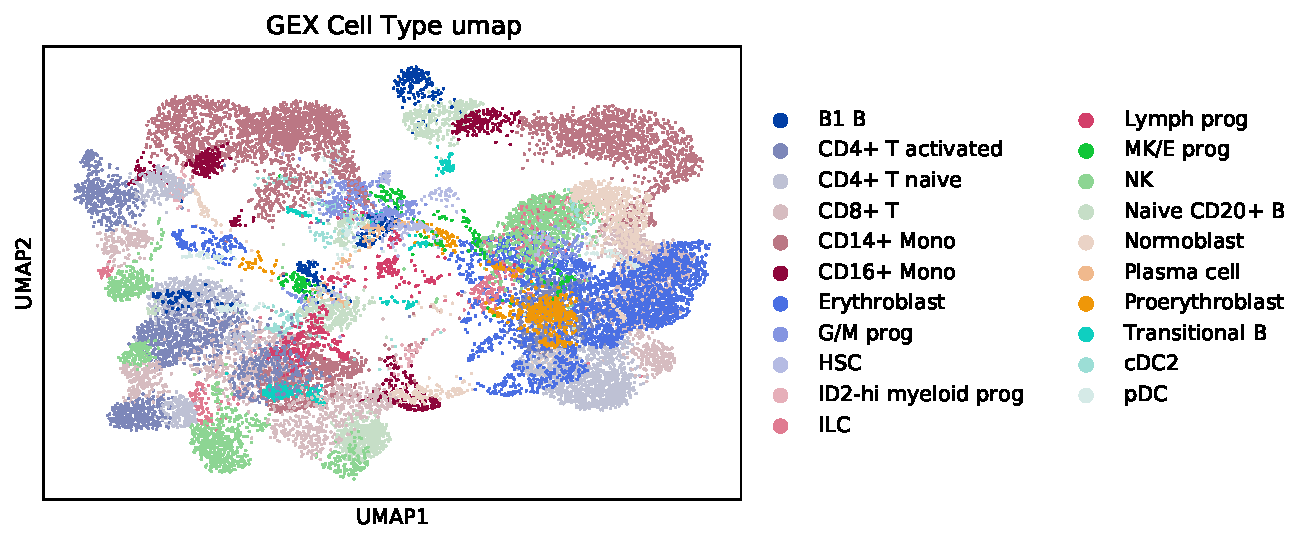
\includegraphics[width=.5\textwidth]{figures/umap_GEX_ct.pdf}
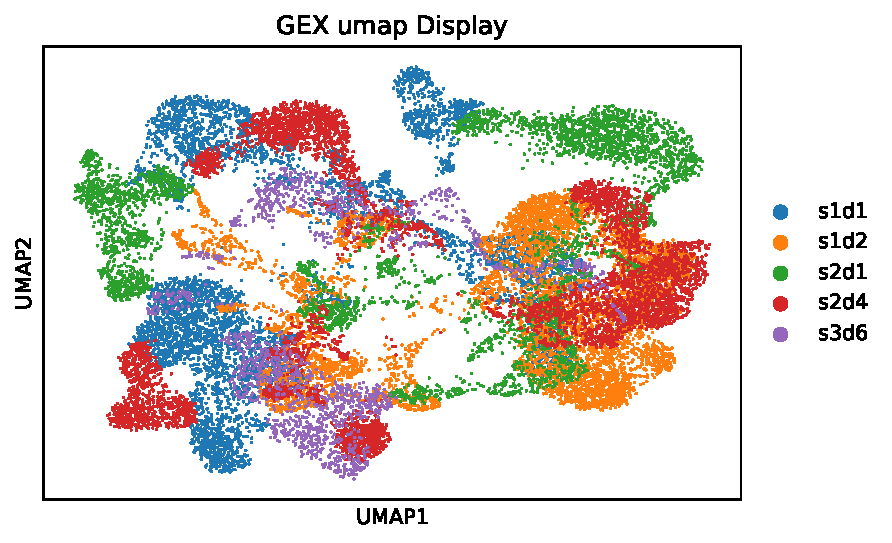
\includegraphics[width=.35\textwidth]{figures/umap_GEX.pdf}
\caption{Left UMAP displays our GEX cell types and our right UMAP displays our source and donors}
\end{figure}

Gene expression analysis has become routine through the development of high-throughput RNA sequencing (RNA-seq) and microarrays. 
RNA analysis that was previously limited to tracing individual transcripts by Northern blots or quantitative PCR is now used frequently to characterize the expression profiles of populations of thousands of cells. 
The data produced from the bulk-based assays has led to the identification of genes that are differentially expressed in distinct cell populations and biomarker discovery. This data comes in the form of \emph{annotated data} (anndata) which is a Python package for handling annotated data matrices in memory and on disk, positioned between pandas and xarray. The numbers within the cell can describe the level of gene expression within a specific immune cell as seen in \textbf{Figure 1}.

\subsection{Assay for Transposase-Accessible Chromatin (ATAC)}

\begin{figure}[H]
\centering
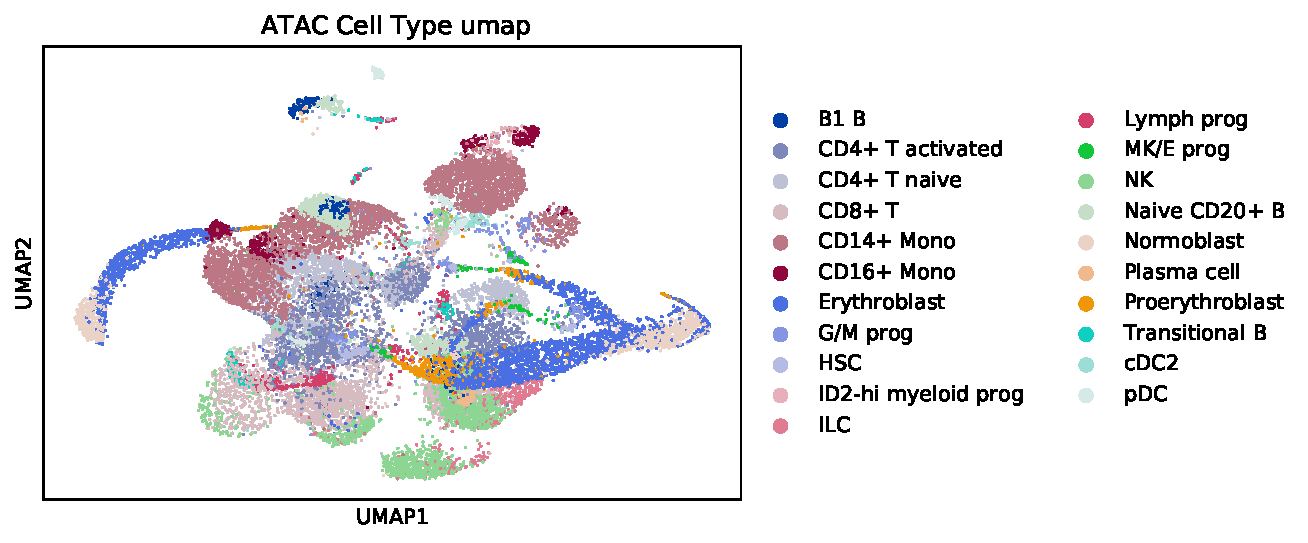
\includegraphics[width=.5\textwidth]{figures/umap_ATAC_ct.pdf}
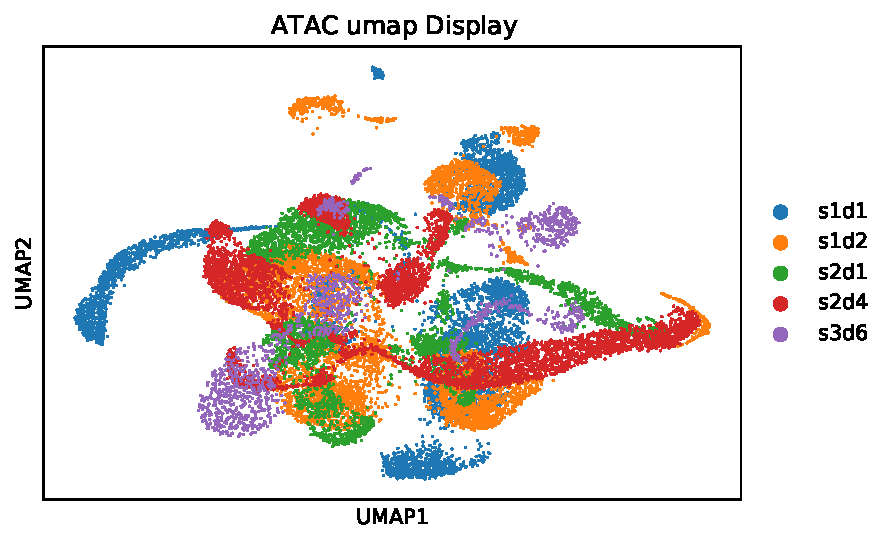
\includegraphics[width=.35\textwidth]{figures/umap_ATAC.pdf}
\caption{Left UMAP displays our ATAC cell types and our right UMAP displays our source and donors}
\end{figure}

Assay for Transposase-Accessible Chromatin or ATAC identifies accessible DNA regions by probing open chromatin with hyperactive mutant Tn5 Transposase that inserts sequencing adapters into open regions of the genome \cite{six}. 
While naturally occurring transposases have a low level of activity, ATAC-seq employs the mutated hyperactive transposase \cite{seven}. 
In a process called "tagmentation", Tn5 transposase cleaves and tags double-stranded DNA with sequencing adaptors \cite{eight}. 
The tagged DNA fragments are then purified, PCR-amplified, and sequenced using next-generation sequencing \cite{eight}.
Sequencing reads can then be used to infer regions of increased accessibility as well as to map regions of transcription factor binding sites and nucleosome positions \cite{six}. 
The number of reads for a region correlates with how open that chromatin is, at single-nucleotide resolution.
This data is also given to us in the form of anndata but unlike the GEX data, the ATAC-seq data comes in binary (e.g. 0,1) to resemble membership of some chromatin within a cell. This property of having binary data will play a huge role in our architecture.

\section{Transformer Attention Model}

\begin{figure}[H]
\centering
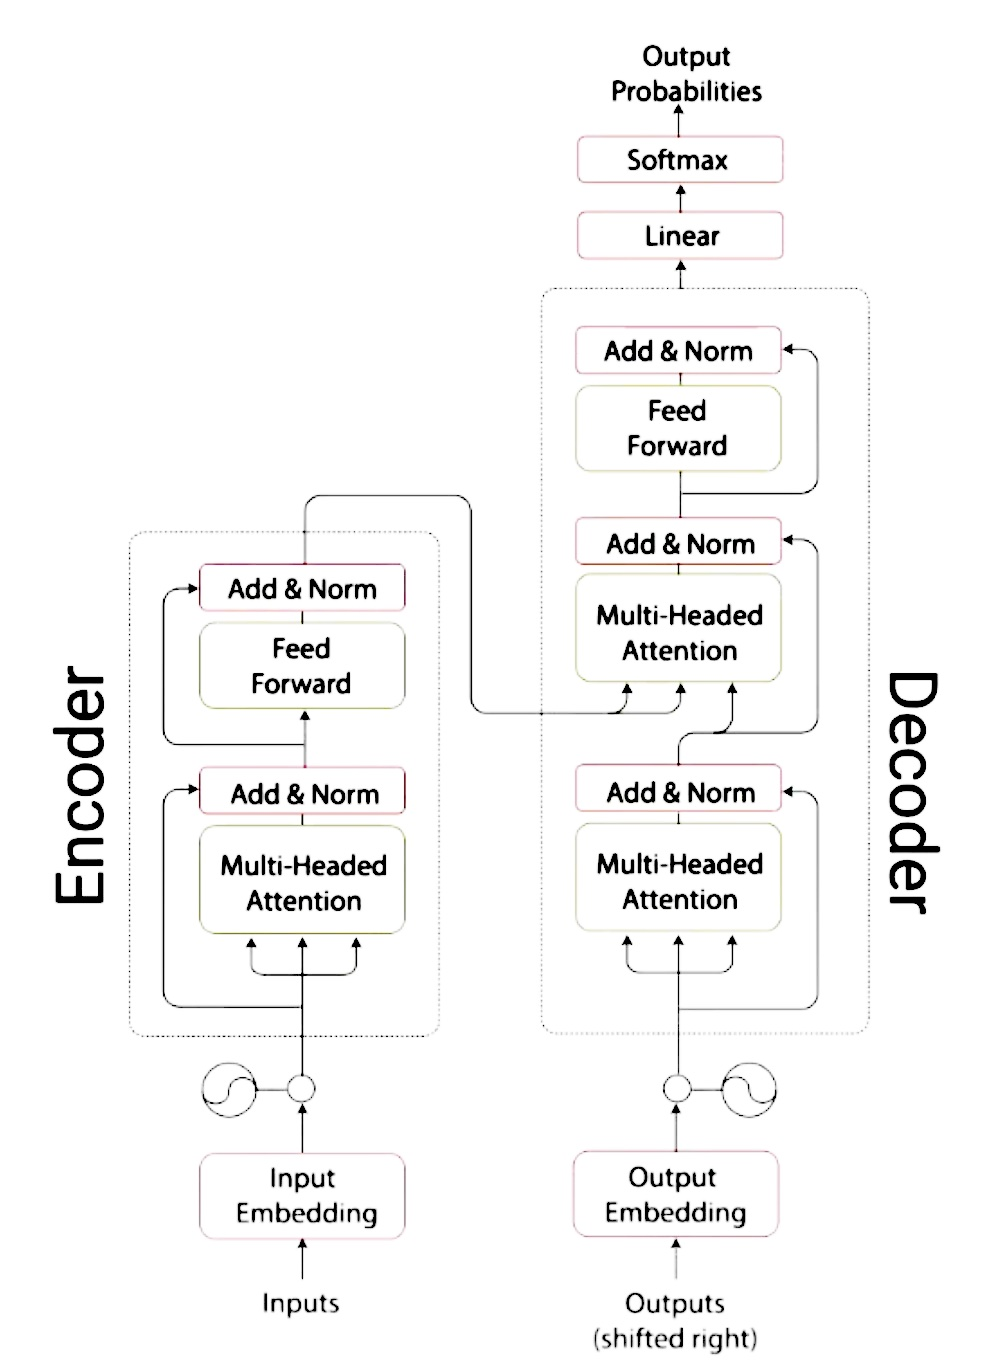
\includegraphics[width=.45\textwidth]{figures/t1.jpg}
\caption{Full architecture on display}
\end{figure}

Transformers are taking the NLP world by storm. These incredible models are breaking multiple NLP records and pushing the state of the art. They are used in many applications like machine language translation, conversational chatbots, and even to power better search engines. To understand transformers we first must revisit the attention mechanism. One of the main advantages of the attention mechanism is its ability to have long-term memory. A transformer model can “attend” or “focus” on all previous tokens (transfer learning) that have been generated. In the following sections, we will describe our model's architecture to help you understand our reasoning for the selection with its brilliance alone. To demonstrate the power of the architecture we will be working with a standard conversational chatbot example to understand the model at a basic level. For this reason, consider the following chatbot conversation:

\begin{figure}[H]
\centering
\textbf{Question:} Hi How are you\\
\textbf{Answer:} I am fine
\end{figure}

\subsection{Encoder}
\noindent
On a high level, the encoders role is standard to those of other neural networks. It maps our input sequence into an abstract continuous representation that holds all the learned information of that input. \\

\noindent
\textbf{Preface. Positional Encoding}

\begin{equation}
\label{Pos Encode}
\text{PE}_{(\text{pos},2i)} = \sin(\frac{\text{pos}}{10000^{\frac{2i}{d_{\text{model}}}}})
\end{equation}

\begin{equation}
\label{Pos Encode2}
\text{PE}_{(\text{pos},2i+1)} = \cos(\frac{\text{pos}}{10000^{\frac{2i}{d_{\text{model}}}}})
\end{equation}

Before getting into the encoders and decoders we first must feed our input into a word embedding layer. A word embedding layer is similar to a lookup table that assigns a unique learned vector representation for each word. Neural networks learn through numbers so each word maps to a vector with continuous values to represent that word. 

Luckily for us, mathematics can be used to make a unique positional encoding for each entry of our input. Some brilliant scientists working on Transformers simply took the properties of the trigonometric functions sine and cosine and made them produce unique values for each positional encoding. As seen in \textbf{Equation 1}, for every odd index on the input vector, create a vector using the cosine function. Similarly in \textbf{Equation 2}, for every even index, we create a vector using the sine function. Then add those vectors to their corresponding input embedding layers. This successfully gives the network information on the position of each vector. 

Now that each word has been given a unique identity, we can proceed to the encoder layer. The Encoders job is to map all input sequences into an abstract continuous representation that holds the learned information for that entire sequence. Within the encoder contains 2 sub-modules, \emph{multi-headed attention}, followed by a fully connected network. There are also residual connections around each of the two sub-layers followed by a layer normalization.\\

\noindent
\textbf{I. Multi-Headed Layer}

\begin{figure}[H]
\centering
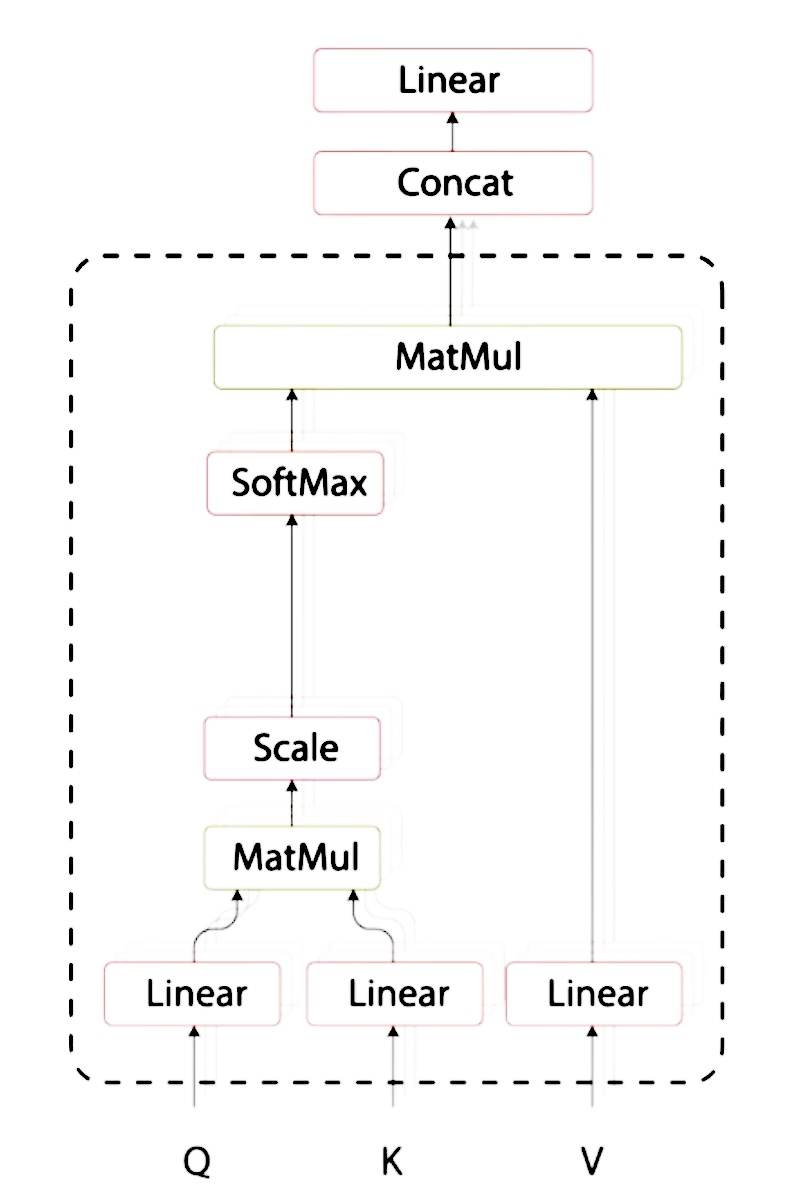
\includegraphics[width=.35\textwidth]{figures/t3.jpg}
\caption{Multi-Headed Layer architecture on display}
\end{figure}

Multi-headed attention in the encoder applies a specific attention mechanism called \emph{self-attention}. \cite{nine} Self-attention is a powerful property that allows the model to associate each word in the input, to other words. So in our conversational chatbot example, our model can learn to associate the word “you”, with “how” and “are”. It is also possible that the model learns to distinguish that words structured in this form are questions that need immediate responses. To achieve self-attention, we feed the input into 3 distinct fully connected layers to create the \emph{query, key}, and \emph{value} vectors.

\begin{figure}[H]
\centering
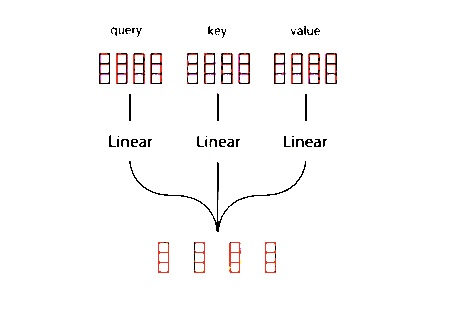
\includegraphics[width=.45\textwidth]{figures/t4.jpg}
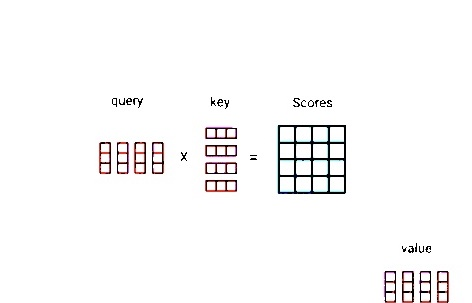
\includegraphics[width=.45\textwidth]{figures/t5.jpg}
\caption{
Left: Our input being set up into query, key and values\\
Right: The dot product between queries and keys
}
\end{figure}

The query key and value concept come from retrieval systems \cite{twelve}.To understand these three important parts, let's take an everyday example of how a \emph{Youtube} search works using this retrieval system. When you type a query to search for some video on \emph{Youtube}, the search engine will compare your query against a set of keys (video title, description, tags, etc.) associated with candidate videos within the database, then present you with the best videos (values) that match your search. 

In the previous section, we defined that we have created a query, key, and value to achieve self-attention. So after creation, we feed the query, key, and value vector through a linear layer, where the queries and keys undergo a dot product matrix multiplication to produce a score matrix as seen in \textbf{Figure 5}. This score matrix determines how much focus should a word be put in comparison to other words. So each word will have a score that corresponds to other words in the time-step. The higher the score the more focus. This is how the queries are mapped to the keys. \textbf{Figure 6} demonstrates our example showing us our score matrix of the conversational chatbot.

\begin{figure}[H]
\centering
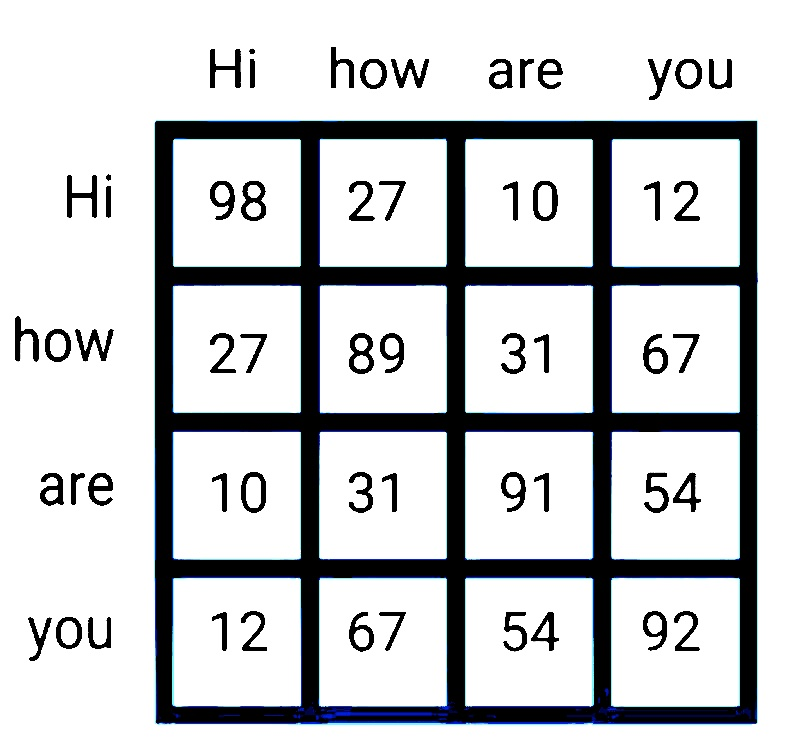
\includegraphics[width=.3\textwidth]{figures/t6.jpg}
\caption{Example Problem - Producing a score matrix}
\end{figure}

However, an issue arises from this as currently constructed. An attention score is not always guaranteed to be a small number and to manage these attention scores within a finite limit we must come up with a clever solution. \\

\newpage
\noindent
\textbf{II. Softmax}

In machine learning, specifically in neural networks, we have a \emph{sigmoid function} denoted by the Greek letter $\sigma$ which is a mathematical function having a characteristic "S"-shaped curve or sigmoid curve. A sigmoid function is simply a logistic function whose y-axis boundaries are bounded within the range $0\leq x \leq 1$ \cite{ten}. Having this unique property of always being within this range has helped machines process much smaller numbers making it much easier to "learn" through the means of backwards propagation.

\begin{figure}[H]
\centering
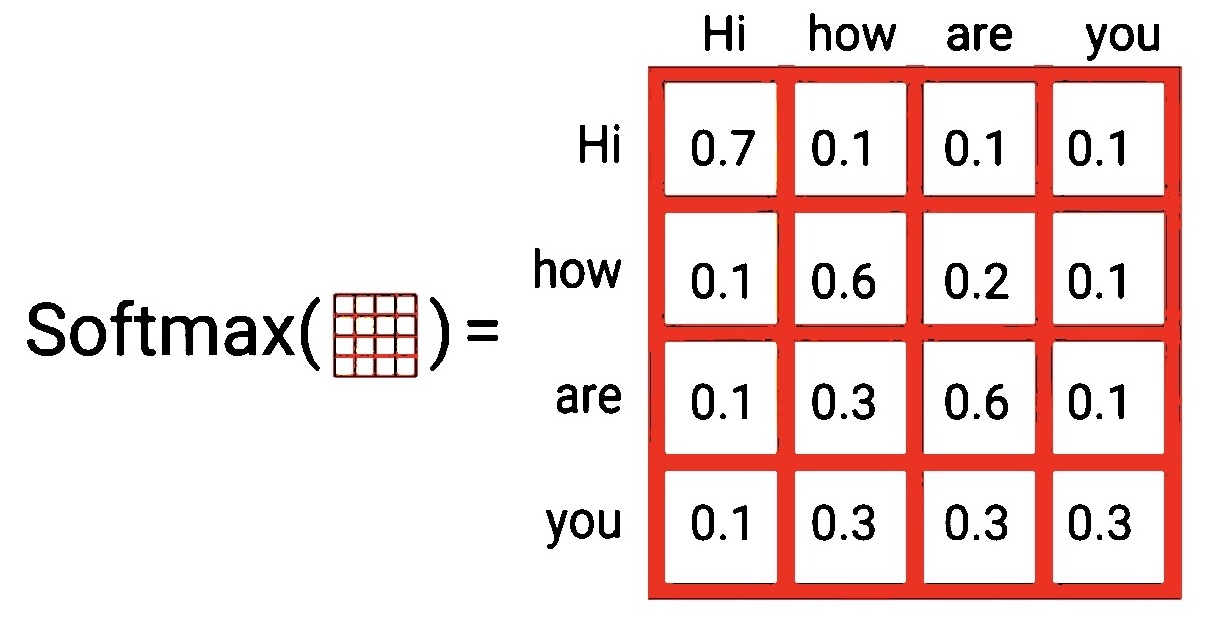
\includegraphics[width=.45\textwidth]{figures/t7.jpg}

\begin{equation}
\label{softmax}
\text{softmax}(x) = \frac{\exp({x_{i}})}{\sum_j \exp({x_{j}})}
\end{equation}

\caption{Scaling down our matrix using the softmax}
\end{figure}

So in our algorithm, we perform a very similar task. Our scores get scaled down in a similar process by dividing the number by the square root of the dimension of query and key. This is to allow for more stable gradients, as multiplying large values can have exploding effects. This process is called applying the \emph{softmax}. Similar to the sigmoid function, once we take the softmax of a matrix, we obtain a scaled-down score with a probability value between 0 and 1 to get the attention weights. By doing a softmax the higher scores get heightened, and lower scores are depressed. This allows the model to be more confident about which words to attend to. 

\begin{figure}[H]
\centering
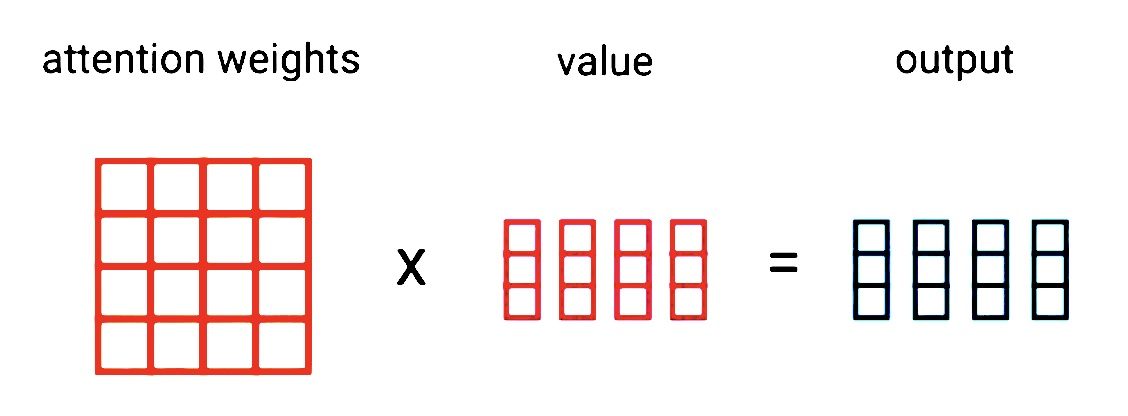
\includegraphics[width=.35\textwidth]{figures/t8.jpg}
\caption{Another dot product between softmax matrix and value vector to obtain output vector}
\end{figure}

Our final process involving the query, keys, and values is to take our attention weights and perform another dot product with the value vector to retrieve an output vector. The higher softmax scores will keep the value of words the model deems as more important. Likewise, the lower scores will drown out the irrelevant words that should not have much focus. Then we feed the output of that into a linear layer to process. So as shown in this example, the algorithm is especially clever in determining how the model attends to specific words. \\

\noindent
\textbf{III. MULTI-headed Layer}

To make this a multi-headed attention computation, you need to split the query, key, and value into $N$ amount of vectors before applying self-attention. The split vectors then go through the self-attention process (the process we just covered) individually. Each self-attention process is called a \emph{head}. Each head produces an output vector that gets concatenated into a single vector before going through the final linear layer. In theory, each head would learn something different therefore giving the encoder model more representation power.

One important question we asked during our development was finding the balance between the number of heads we wish to compute versus the accuracy of our attention-based neural network. In theory, the increased numbers in heads would only benefit the model's ability to learn, however at what point was this model too taxing and computationally slow to be considered a good model. Because we intend to work with a data set that needs to process hundreds of millions of cell data, at what point were we to decide how many heads we should compute for our particular model. We feared that if we had "too little" heads, that our model would not be a very good predictor. So as we move forward we wanted to acknowledge this particular question we had during our development. 

\begin{figure}[H]
\centering
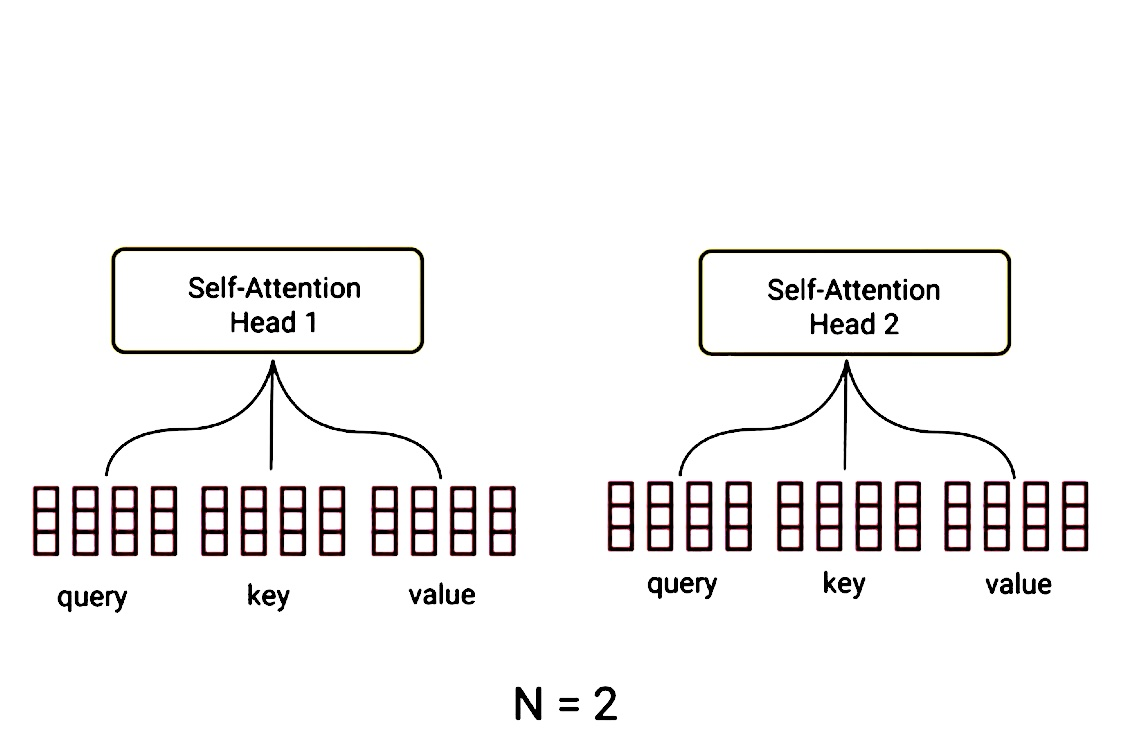
\includegraphics[width=.4\textwidth]{figures/t9.jpg}
\caption{Multi-Headed Layer split into N = 2 "heads"}
\end{figure}

To sum it up, multi-headed attention is a module in the transformer network that computes the attention weights for the input and produces an output vector with encoded information on how each word should attend to all other words in that particular sequence. \\

\noindent
\textbf{IV. The Residual Connections, Layer Normalization, and Feed Forward Network}

Next, the multi-headed attention output vector that we just computed is added to the original positional input embedding. This process is called a \emph{residual connection}. The output of the residual connection goes through a layer normalization. 

\begin{figure}[H]
\centering
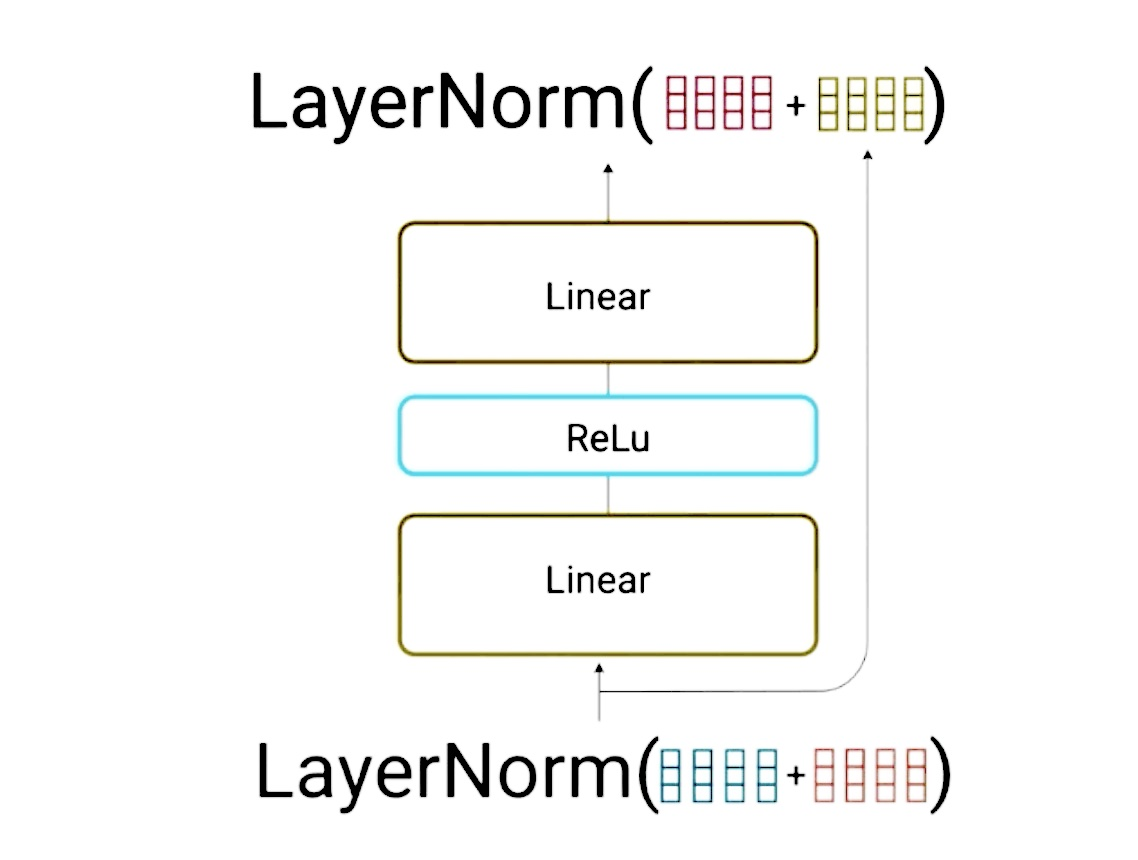
\includegraphics[width=.4\textwidth]{figures/t10.jpg}
\caption{Layer Normalization}
\end{figure}

Inside the layer normalization, the residual output gets projected through a point-wise feed-forward network for further processing. The point-wise feed-forward network is a couple of linear layers with a Rectified Linear Unit (ReLU) activation in between. In the context of neural networks, ReLU activation function\cite{eleven} is an activation function defined as the positive part of its argument: where x is the input to a neuron.

\begin{equation}
\label{softmax}
f(x) = x^{+} = \text{max}(0,x)
\end{equation}

\newpage
\noindent
In mathematical terms a ReLU activation function can be described as a piecewise linear function that will output the input directly if it is positive, otherwise, it will output zero. The rectified linear activation function overcomes the vanishing gradient problem, allowing models to learn faster and perform better.

Now going back to the point-wise feed-forward network, the output of that is then again added to the input of the point-wise feed-forward network and further normalized. The residual connections help the network train, by allowing gradients to flow through the networks directly. The layer normalizations are used to stabilize the network which results in substantially reducing the training time necessary. The point-wise feed-forward layer is used to project the attention outputs potentially giving it a richer abstract representation. \\

\noindent
\textbf{V. Encoder Final Remarks}

With that, that wraps up the encoder layer. All of these operations are to encode the input to a continuous representation with attention information. This will help the decoder focus on the appropriate words in the input during the decoding process. You can stack the encoder N times to further encode the information, where each layer has the opportunity to learn different attention representations therefore potentially boosting the predictive power of the transformer network.

\subsection{Decoder}

\begin{figure}[H]
\centering
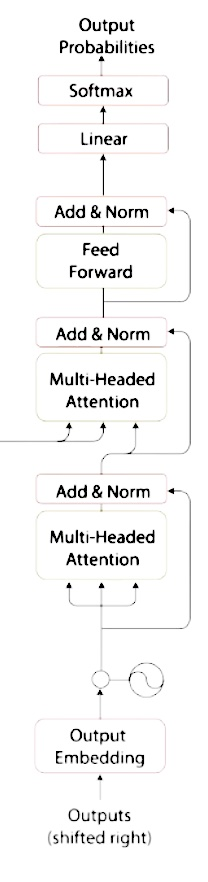
\includegraphics[width=.14\textwidth]{figures/t11.jpg}
\caption{Decoder Architecture}
\end{figure}

The decoder’s job is to generate text sequences from the abstract representation containing attention information. To our surprise, the decoder has a similar architecture in terms of its sub-layer as the encoder. It has two multi-headed attention layers, a point-wise feed-forward layer, and residual connections, and layer normalization after each sub-layer. These sub-layers behave similarly to the layers in the encoder but each multi-headed attention layer has a different job. The decoder is capped off with a linear layer that acts as a classifier, and a softmax to get the word probabilities. So on a high level, the decoder's role is to take our continuous representation and step by step generates a single output while also being fed the previous output.

The decoder is \emph{auto-regressive} meaning it begins with a start token, and it takes in a list of previous outputs as inputs, as well as the encoder outputs that contain the attention information from the input. The decoder stops decoding when it generates a token as an output. \\

\noindent
\textbf{I. Multi-Headed Layer}

As mentioned in the introduction the primary difference occurs within the multi-headed layer. Since the decoder is auto-regressive and generates the sequence word by word, you need to prevent it from conditioning the future tokens. For example, when computing attention scores on the word “am”, you should not have access to the word “fine”, because that word is a future word that was generated after. The word “am” should only have access to itself and the words before it. This is true for all other words, where they can only attend to previous words.

\begin{figure}[H]
\centering
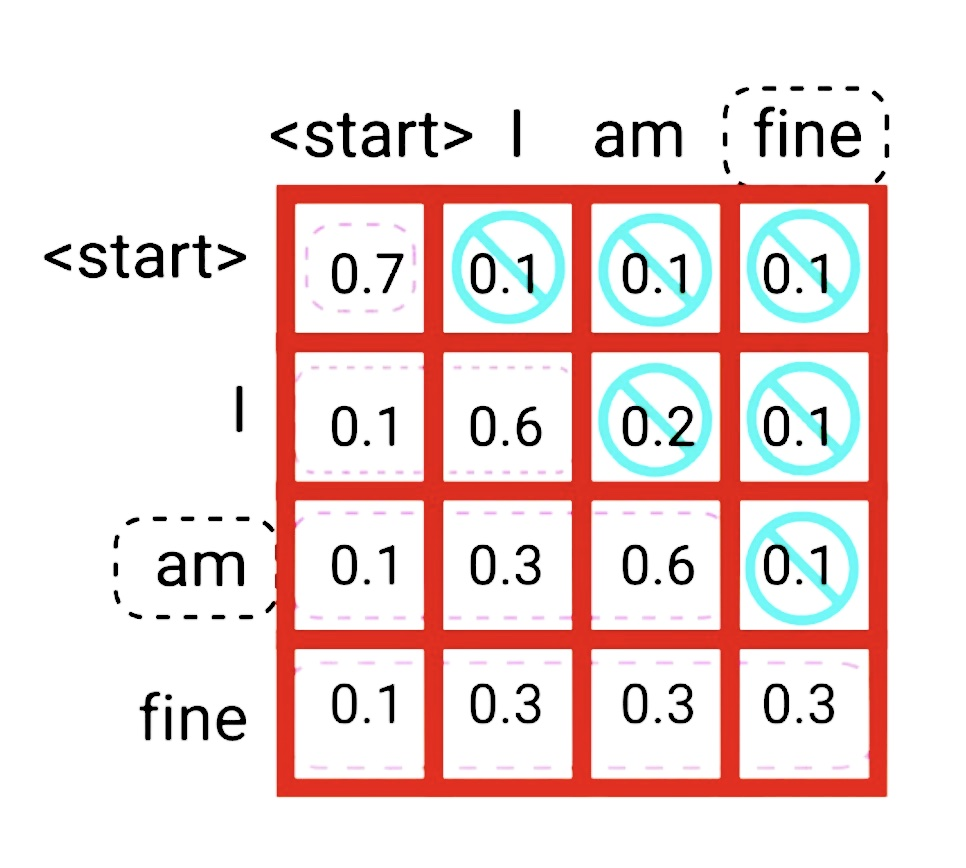
\includegraphics[width=.3\textwidth]{figures/t12.jpg}
\caption{Multi-Headed Layer shouldn't access future tokens}
\end{figure}

As a result, we need a method to prevent the issue of computing attention scores for future words. Therefore we use a method called \emph{masking}. To prevent the decoder from looking at future tokens, you apply a look-ahead mask. The mask is added before calculating the softmax, and after scaling the scores. \\

\noindent
\textbf{II. Look Ahead Mask}

\begin{figure}[H]
\centering
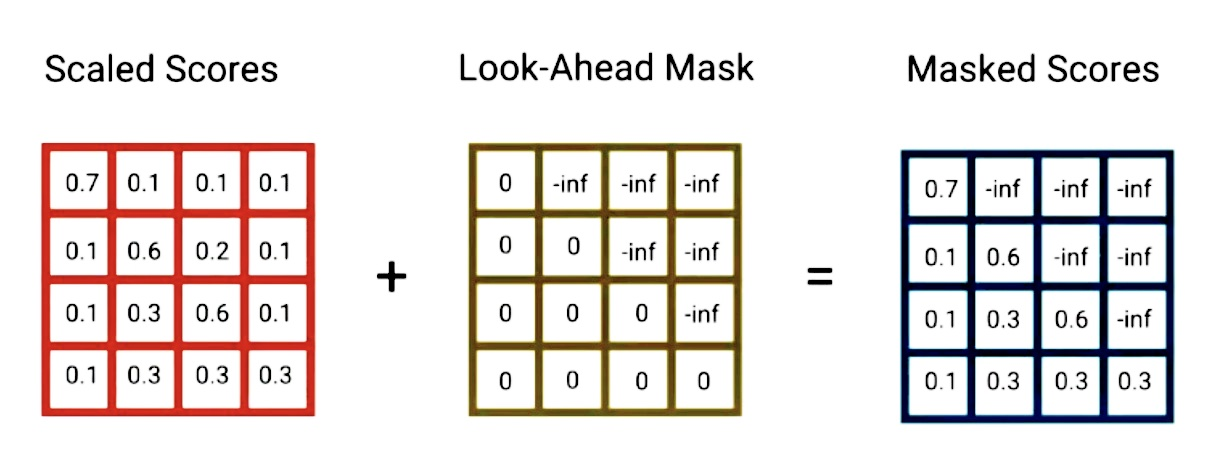
\includegraphics[width=.55\textwidth]{figures/t13.jpg}
\caption{Scaled scores being added to the look ahead mask to retrieve a matrix of masked scores}
\end{figure}

The look-ahead mask is a matrix that’s the same size as the attention scores filled with values of 0’s and/or negative infinities. When you add the mask to the scaled attention scores, you get a matrix of the scores, with the top right triangle filled with negativity infinities as shown in \textbf{Figure 13}. Adding these two sets of matrices together helps us obtain our masked scores.

\begin{figure}[H]
\centering
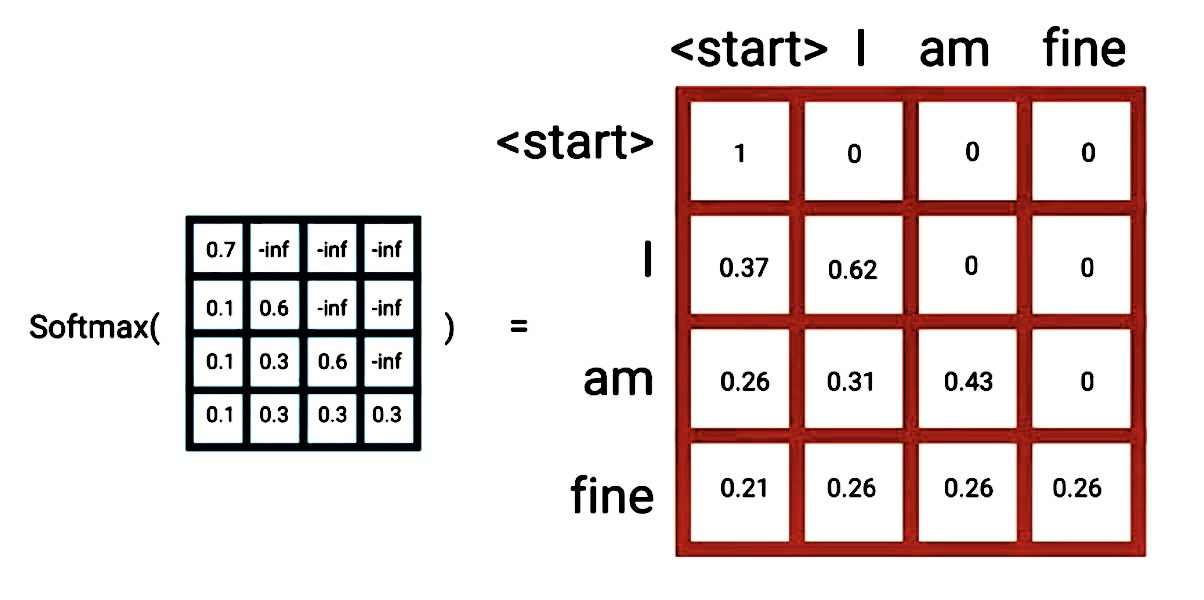
\includegraphics[width=.3\textwidth]{figures/t14.jpg}
\caption{Softmaxing the masked scores}
\end{figure}
\newpage


The reason for the mask is because once you take the softmax of the masked scores, the negative infinities get zeroed out, leaving zero attention scores for future tokens. As you can see in the \textbf{Figure 14}, the attention scores for “am”, has values for itself and all words before it but is zero for the word “fine”. This essentially tells the model to put no focus on those words.

This masking is the only difference in how the attention scores are calculated in the first multi-headed attention layer. This layer still has multiple heads, that the mask is being applied to, before getting concatenated and fed through a linear layer for further processing. The output of the first multi-headed attention is a masked output vector with information on how the model should attend to the decoder’s input. \\

\noindent
\textbf{III. Second Multi-Headed Layer}

For this layer, the encoder’s outputs are the queries and the keys, and the first multi-headed attention layer outputs are the values. This process matches the encoder’s input to the decoder’s input, allowing the decoder to decide which encoder input is relevant to put a focus on. The output of the second multi-headed attention goes through a point-wise feed-forward layer for further processing.\\

\noindent
\textbf{IV. Linear Classifier and Final Softmax for Output Probabilities}

The output of the final point-wise feed-forward layer goes through a final linear layer, that acts as a classifier. The classifier is as big as the number of classes you have. For example, if you have 10,000 classes for 10,000 words, the output of that classier will be of size 10,000. The output of the classifier then gets fed into a softmax layer, which will produce probability scores between 0 and 1. We take the index of the highest probability score, and that equals our predicted word.

\begin{figure}[H]
\centering
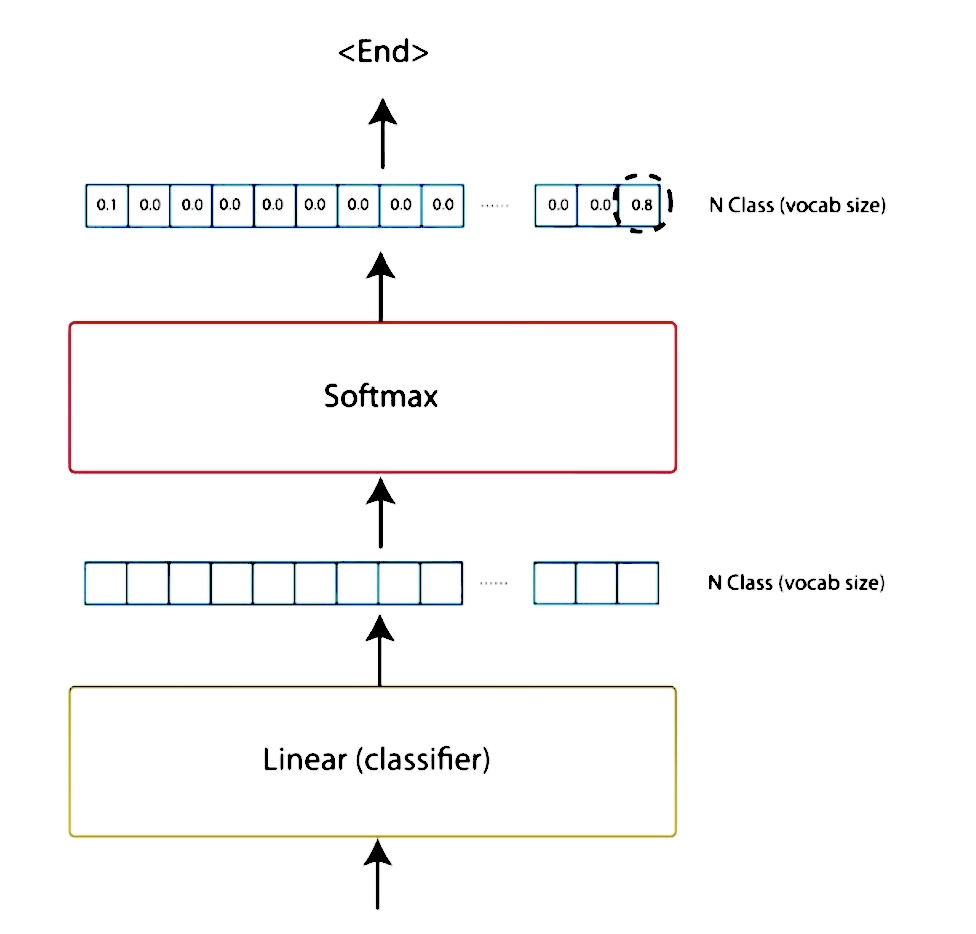
\includegraphics[width=.55\textwidth]{figures/t15.jpg}
\caption{Last steps in decoder to properly determine the predicted word}
\end{figure}

The decoder then takes the output, add’s it to the list of decoder inputs, and continues decoding again until a token is predicted. For our case, the highest probability prediction is the final class which is assigned to the end token.

The decoder can also be stacked N layers high, each layer taking in inputs from the encoder and the layers before it. By stacking the layers, the model can learn to extract and focus on different combinations of attention from its attention heads, potentially boosting its predictive power.
\newpage

\section{Preprocessing \& Training}

In this section, we will discuss the parameters we decided to change for our biology-based problem. As it currently stands this model will not necessarily work because our data is not properly prepared to be fed into the \emph{t5-small}. With our main objective to be able to map GEX to ATAC-seq data and vice versa, there are potential architectural issues we had to address in order to make this work. Our design will be discussed in this section.

\subsection{Data Preprocessing: Binarizing our Data}

\begin{figure}[H]
\centering
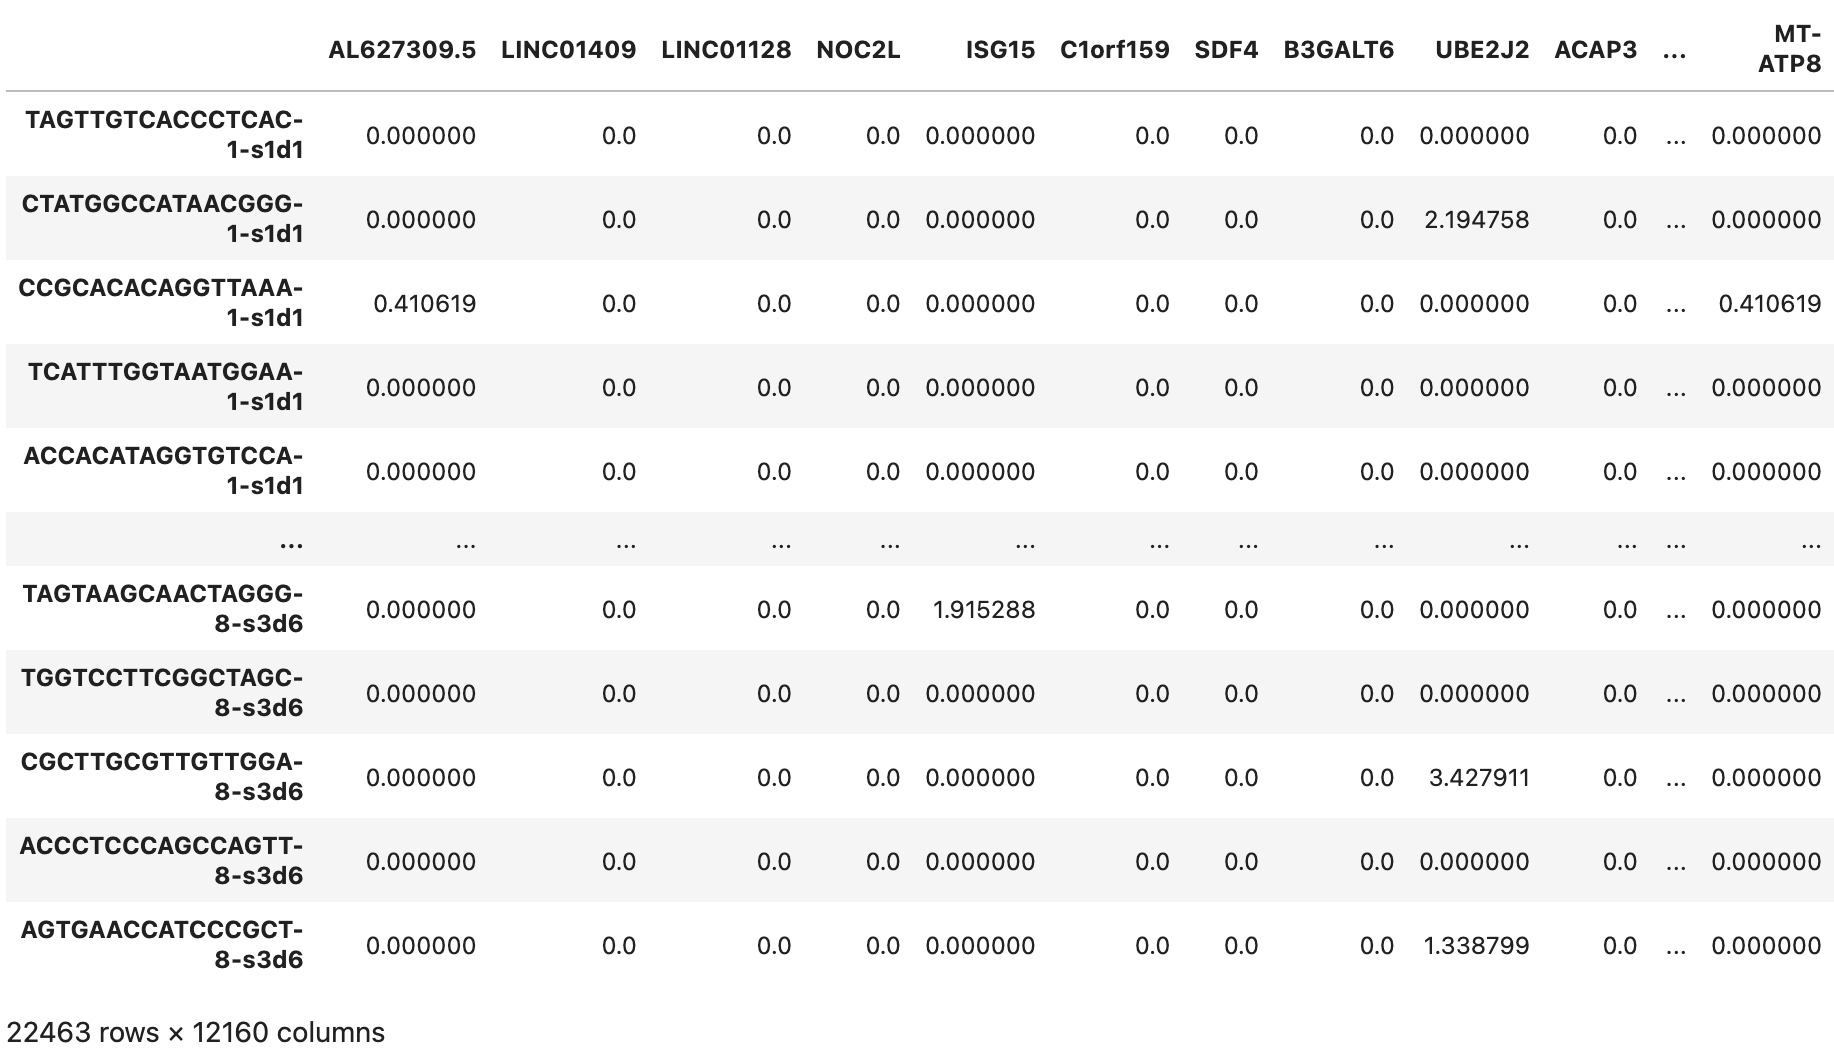
\includegraphics[width=.85\textwidth]{figures/gexdata.jpg}
\caption{Our GEX data}
\end{figure}

One of the primary issues that currently stand is that our data is not "legible". If we were to feed the data into our model without any edits, it would most definitely fail because our transformer model does not know how to extract data from the anndata matrix. Anndata is a rather hard data structure to work with overall because it is hard to manipulate the entries of the matrix. Its primary purpose is to just have a scalable way of keeping track of data and its learned annotations. Therefore one of the first changes we made was converting our anndata into a NumPy array. Our decision to change our matrix data structure was influenced by the fact that it is much easier to manipulate any size matrix easily with the built-in tools of NumPy. 

Although we are now able to manipulate the entries of the matrix more familiarly, we still have not fixed the legibility issue. It is indeed true that neural networks learn from numbers but what good will feeding a float number do for our neural network in the training process. For example in our GEX data at row 2, we can see that CTATGGCCATACGGG-1-s1d1 has expressed the gene UBE2J2 at 2.194758. However what valuable information does our model grasp in this process? While we don't have an exact answer, we can assume it will learn nothing because there are no patterns found within the float numbers alone. So to overcome this issue we came up with a high risk low reward solution. 

Our ATAC-seq anndata was presented to us in a binary form. Traditionally binary has been used to express whether something has membership into a specific group. Therefore to pass in strings instead of integers and floats, we decided to binarize our GEX data. However, it is important to acknowledge that by doing this, we most definitely lose out on some important information. But by binarizing our data we can extract the specific gene expression and/or chromatin in its string form to pass it in as a python dictionary for preprocessing. We set the threshold to be over/under 2.0 meaning that if the gene expressed was under 2.0 it would be converted to 0 and if it was 2.0 or above it would be converted into 1. In our example, the CTATGGCCATACGGG-1-s1d1 which expressed the gene UBE2J2 at 2.194758 would be converted to a 1 because 2.194758 is greater than 2.0. So while we think this is a witty solution, we also know that gene expression is not a one-dimensional measurement and we lose some important information in the process. 

\subsection{Data Preprocessing: Setting up our input}

Now that our data is binarized, the second part of the preprocessing is to get our data ready to be fed into our Transformer attention model. As mentioned in the previous section, the primary motivation on converting our data into binary was to express membership to a group. In our case it is to express membership to a certain gene being expressed or a chromatin location at which it occurs. Knowing this information we just came up with a solution in the previous section to pass in strings as input versus the integers and floats. Because the transformer is a NLP model it was important that we made our input into strings so that our model could properly learn in the process. 

\begin{equation}
\textbf{\{{\text{'En': 'That is good.'}}, {{\text{'De': 'Das ist gut.'}}\}}}
\end{equation}

\begin{equation}
\textbf{\{ \text{'TAGGTA': 'chr1-633515 chr1-633525 '},  \text{'TAGGTA': 'MT-ND3 MT-ND4 MT-CYB '}\}}
\end{equation}

The transformer takes in input through the use of Python dictionaries. Python Dictionaries are quite the intuitive design because they come with a key and a value. The key is typically some label that we can use to identify a certain entry and the value is some quantity or text that is associated with the key. So in \textbf{(5)} we can see a NLP example. In this example, the keys are the languages in which we want to perform a machine translation and the values are the English and German phrases that correspond to each other. Similarly, in \textbf{(6)} the key resembles the cell name and the value is the gene being expressed and the chromatin location. To get all cells with their associated GEX and ATAC-seq dictionaries we made a python function that traversed the whole matrix and extracted the text if and only if their binary value was switched to 1. Though this computation is rather slow we have had conversations about using a sparse matrix in the future to combat this slow computational speed. However, in our first version of the model, we have decided to let our computer simply take as much time as it needed to get our dictionaries set up. 

\begin{figure}[H]
\centering
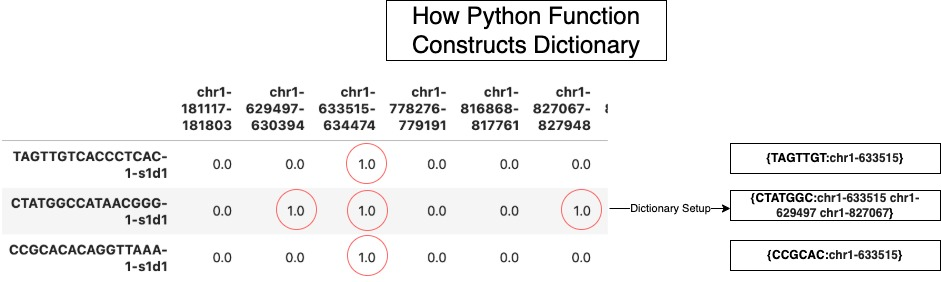
\includegraphics[width=.85\textwidth]{figures/pyfunc.jpg}
\caption{Dictionary Construction}
\end{figure}

\noindent
After creating all the dictionaries for each individual cell we stored them into a .txt file as a place to hold all information. By doing so we have completed the preprocessing portion for our multi-modal predictor program.

\subsection{Training}

At last, we look to begin training our model. Because the \emph{t5-small} is a well-established model from \emph{Google}, we simply had to pip install all the model's packages as well as import them into our code and begin the training process. Because the t5-small was a pre-trained model, we had to retrain this model from scratch. What that means for us is that our model relies solely on the 22,463 cells to build its intuition even with the sparsity of our data. When a data set is sparse it means that the majority of the matrix data are filled with zeros. In our scATAC-seq and GEX matrices, only about 3\% of our entries were non-zero. So while we have a decent-sized matrix of 22,463 different types of cells, this may be slightly deficient for completely accurate predictions.  

\section{Preliminary Results}

After the completion of our training, our model, in theory, is ready for use. So as a result we designed a test using some conference-level code vs our t5-small transformer model. The purpose of these tests was to run a series of tests and get an approximate value that assesses the accuracy of the prediction. We pulled 4 models designed for multi-modality prediction from the NeurIPS Conference. All these models are designed to use different machine learning designs that perform the same task as our model. These 4 models are the \emph{KAUST, Cajal, Dengkw,} and the \emph{DANCE} \cite{thirteen}. 

\begin{figure}[H]
\centering
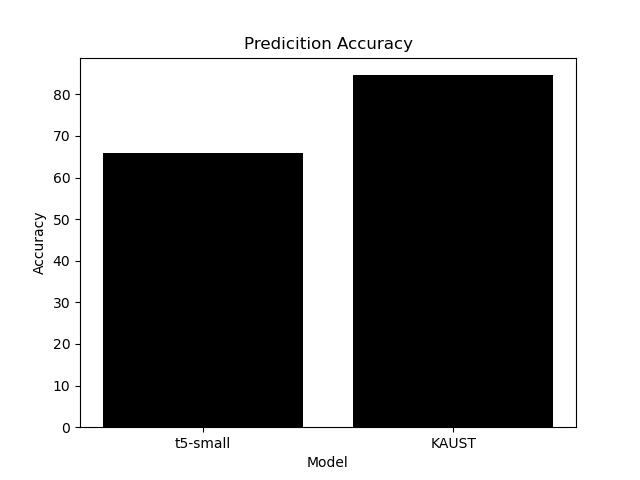
\includegraphics[width=.4\textwidth]{figures/data1.png}
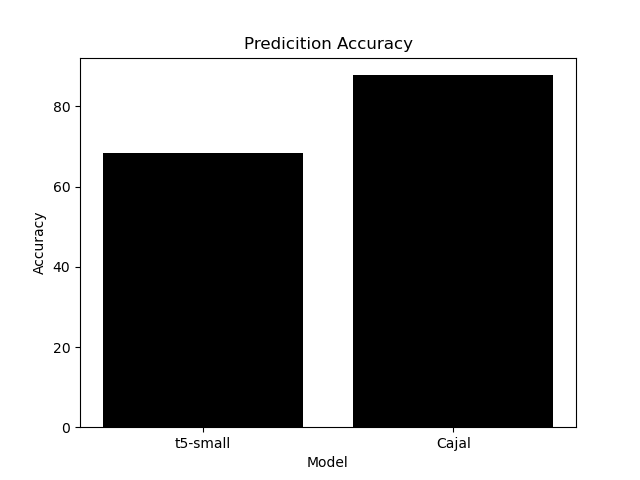
\includegraphics[width=.4\textwidth]{figures/data2.png}\\
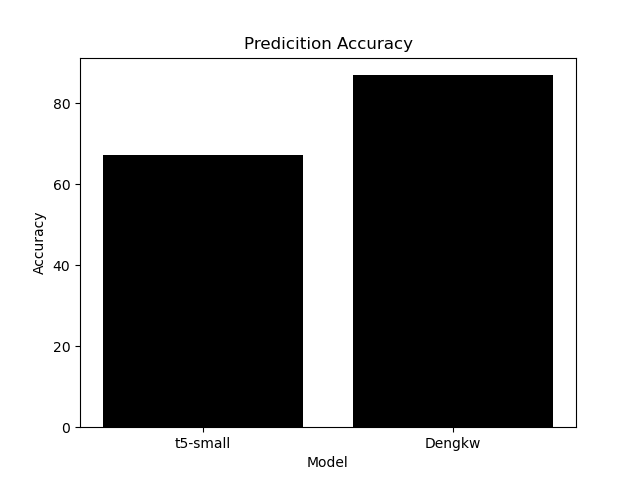
\includegraphics[width=.4\textwidth]{figures/data3.png}
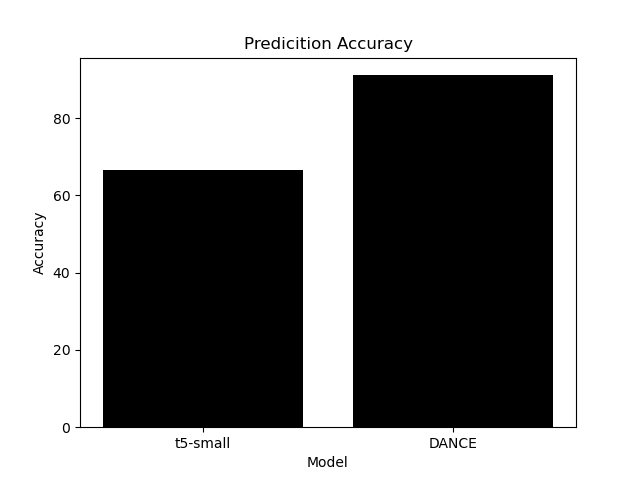
\includegraphics[width=.4\textwidth]{figures/data4.png}
\caption{Prediction percentages lined up against conference code}
\end{figure}


All the models presented in these experiments are a two-way system. Therefore we designed a test that assessed the accuracy by running 500 different inputs: 
250 ATAC->GEX \& 250 GEX->ATAC. Through this, we got preliminary results as presented in \textbf{Figure 18}. Our model's accuracy for its predictions lies within the range 65\% and 70\%. Meanwhile some of the code from the other lies within the 80\% to 90\% range. While there tends to be a noticeable gap, we have previously mentioned why this appears to be the case. 

\begin{table}[h!]
\centering
 \begin{tabular}{||c | c | c||} 
 \hline
 Model & t5-small & Opposing Model \\ [0.5ex] 
 \hline\hline
 KAUST & 65.8 & 84.6  \\ 
 Cajal & 68.3 & 87.8  \\
 Dengkw & 67.3 & 86.9  \\
 DANCE & 66.5 & 91.1  \\ [1ex]
 \hline
 \end{tabular}
\end{table}

Our model loses a significant amount of important GEX data when we decided to binarize our data during the preprocessing. Our reasoning for this binarization was based solely on the way we constructed the data to be trained. Because we wanted to express membership to obtain the name we decided to choose a threshold of 2.0 and make that as a way to determine which cells are flipped to 0 and 1's. So while our model can perform really well in the ATAC->GEX prediction, it lacks a little in the GEX->ATAC. We ran this test on the t5-small on 4 different occasions to see how it would match up with the model it was competing against and we saw a high of 68.3\% accuracy and a low of 65.8\%. While the model is not perfect, we can say that this model was no doubt successful. By taking a novel approach using an NLP-based tool and using it in a biological problem, there was no doubt that we would experience some trouble in the process. However, we believe that our prototype model has the potential to be a viable method using single-cell analyses across all modalities.  

\section{Conclusion}

The t5-small transformer model by Google can officially now add predicting scRNA-seq modalities from one another into its list of functional tasks.  While we have seen ample progress throughout this research, we must acknowledge as well the deficiencies
that currently exist and where we will go from here.

In terms of our lost data in the preprocessing process, we will work towards finding a more clever solution that may not lose out on Gene expression data as we have identified GEX to be more than one-dimensional. Additionally, we also are trying to find ways to optimize the data preparation and preprocessing of this model. Constructing roughly 22,000 python dictionaries that are relocated into .txt files served to be an extremely slow process. However with our lab containing mathematicians who study algorithmic development we have already thought of ways to optimize our code through the use of sparse matrices to limit the extreme matrix space that we are asked to work with. Therefore through it all, we have seen promise in our model and will continue to look for ways to optimize and work with a more complex representation of our data. With scRNA-seq still being a very active form of research, our expectation is that we will see more data science tools coming from all different fields of machine learning to be soon implemented into biological data analyses.

\section{Acknowledgement}



\begin{thebibliography}{25}

\bibitem{one} Zhang, J., Chiodini, R., Badr, A., \& Zhang, G. (2011). "The impact of next-generation sequencing on genomics". Journal of genetics and genomics = Yi chuan xue bao, 38(3), 95–109. https://doi.org/10.1016/j.jgg.2011.02.003

\bibitem{two} Janocha, K., Czarnecki, W. M. (2017). "On loss functions for deep neural networks in classification". Retrieved August 2, 2020, from the arXiv database.

\bibitem{three} Nadkarni, P. M., Ohno-Machado, L., \& Chapman, W. W. (2011). "Natural language processing: an introduction". Journal of the American Medical Informatics Association: JAMIA, 18(5), 544–551. https://doi.org/10.1136/amiajnl-2011-000464

\bibitem{four} Raffel, C., Shazeer, N., Roberts, A., Lee, K., Narang, S., Matena, M., Zhou, Y., Li, W. and Liu, P.J., (2019). "Exploring the limits of transfer learning with a unified text-to-text transformer". arXiv preprint arXiv:1910.10683.

\bibitem{five} Luecken, M.D., Burkhardt, D.B., Cannoodt, R., Lance, C., Agrawal, A., Aliee, H., Chen, A.T., Deconinck, L., Detweiler, A.M., Granados, A.A. and Huynh, S., (2021). "A sandbox for prediction and integration of dna, rna, and proteins in single cells." In Thirty-fifth Conference on Neural Information Processing Systems Datasets and Benchmarks Track (Round 2).

\bibitem{six} Buenrostro JD, Wu B, Chang HY, Greenleaf WJ (2015). "ATAC-seq: A Method for Assaying Chromatin Accessibility Genome-Wide". Current Protocols in Molecular Biology. 109: 21.29.1–21.29.9. doi:10.1002/0471142727.mb2129s109. PMC 4374986. PMID 25559105.

\bibitem{seven} Reznikoff WS (2008). "Transposon Tn5". Annual Review of Genetics. 42 (1): 269–86. doi:10.1146/annurev.genet.42.110807.091656. PMID 18680433.

\bibitem{eight} Picelli S, Björklund AK, Reinius B, Sagasser S, Winberg G, Sandberg R (2014). "Tn5 transposase and tagmentation procedures for massively scaled sequencing projects". Genome Research. 24 (12): 2033–40. doi:10.1101/gr.177881.114. PMC 4248319. PMID 25079858.

\bibitem{nine} Vaswani, A., Shazeer, N., Parmar, N., Uszkoreit, J., Jones, L., Gomez, A.N., Kaiser, Ł. and Polosukhin, I., (2017). Attention is all you need. In Advances in neural information processing systems (pp. 5998-6008).

\bibitem{ten} Han, J., Morag, C (1995). "The influence of the sigmoid function parameters on the speed of backpropagation learning". In Mira, José; Sandoval, Francisco (eds.). From Natural to Artificial Neural Computation. Lecture Notes in Computer Science. 930. pp. 195–201. doi:10.1007/3-540-59497-3\_175. ISBN 978-3-540-59497-0.

\bibitem{eleven} Brownlee, J (2019). "A Gentle Introduction to the Rectified Linear Unit (ReLU)". Machine Learning Mastery. Retrieved 8 April 2021.

\bibitem{twelve} Jansen, B. J. and Rieh, S. (2010) "The Seventeen Theoretical Constructs of Information Searching and Information Retrieval Archived 2016-03-04 at the Wayback Machine." Journal of the American Society for Information Sciences and Technology. 61(8), 1517-1534.

\bibitem{thirteen} https://github.com/openproblems-bio/neurips2021\_multimodal\_topmethods

\end{thebibliography}
